

\section{Evaluation}
\label{sec:evaluation}

% \subsection{Evaluation of Base Models}

As illustrated above, GLM-5 marks the transition from vibe coding to a new era of agentic engineering. 
We first assess GLM-5 with frontier models on agentic, reasoning, and coding (ARC) benchmarks. 
To fully evaluate the performance of GLM-5 in real-world agentic engineering scenarios, we propose a new internal evaluation suite, CC-Bench-V2, which includes frontend, backend, and long-horizon tasks. 
Finally, we evaluate the general abilities of GLM-5 in five common real-world scenarios. 


\subsection{Evaluation of ARC Benchmarks}

We report the main results of the ARC benchmarks in Table~\ref{tab:eval_arc} that compare GLM-5 with GLM-4.7, DeepSeek-V3.2~\cite{liu2025deepseek}, Kimi-K2.5~\cite{team2026kimi}, Claude Opus 4.5~\cite{opus4.5}, Gemini 3 Pro~\cite{gemini3}, and GPT-5.2 (xhigh)~\cite{gpt-5.2}. 
In general, GLM-5 delivers a significant improvement over GLM-4.7 and achieves state-of-the-art performance among open-source models, narrowing the gap to proprietary models such as Claude Opus 4.5. Evaluation details can be found at Section~\ref{sec:eval_details_arc}.

\begin{table}[htbp]
\centering
\caption{\label{tab:eval_arc} Comparison between GLM-5 and open-source/proprietary models. Results marked with * are from the full set of HLE. Results marked with $^\dagger$ are evaluated on a verified version of Terminal-Bench 2.0, fixing some ambiguous instructions. The GDPval-AA Elo scores are recorded on 15th Feb., 2026. The highest score for each benchmark is \textbf{bolded}, and the second highest is \underline{underlined}.}
\setlength{\tabcolsep}{3pt}
\renewcommand{\arraystretch}{1.15}
\begin{tabular}{lccccccc}
\toprule
& \textbf{GLM-5} & \textbf{GLM-4.7} & \begin{tabular}[c]{@{}c@{}}\textbf{DeepSeek}\\\textbf{-V3.2}\end{tabular} & \begin{tabular}[c]{@{}c@{}}\textbf{Kimi}\\\textbf{K2.5}\end{tabular} & \begin{tabular}[c]{@{}c@{}}\textbf{Claude}\\\textbf{Opus 4.5}\end{tabular} & \begin{tabular}[c]{@{}c@{}}\textbf{Gemini}\\\textbf{3 Pro}\end{tabular} & \begin{tabular}[c]{@{}c@{}}\textbf{GPT-5.2}\\\textbf{(xhigh)}\end{tabular}  \\
\midrule
\textit{Reasoning \& General} & & & & & & & \\
HLE & 30.5 & 24.8 & 25.1 & 31.5 & 28.4 & \textbf{37.2} & \underline{35.4} \\
HLE (w/ Tools) & \underline{50.4} & 42.8 & 40.8 & \textbf{51.8} & 43.4* & 45.8* & 45.5* \\
AIME 2026 I & 92.7 & \underline{92.9} & 92.7 & 92.5 & \textbf{93.3} & 90.6 & - \\

HMMT Feb. 2025 & \underline{97.9} & 97.1 & 92.5 & 95.4 & 92.9 & 97.3 & \textbf{99.4} \\
HMMT Nov. 2025 & \underline{96.9} & 93.5 & 90.2 & 91.1 & 91.7 & 93.0 & \textbf{97.1} \\
IMO-AnswerBench & 82.5 & 82.0 & 78.3 & 81.8 & 78.5 & \underline{83.3} & \textbf{86.3} \\
GPQA-Diamond & 86.0 & 85.7 & 82.4 & 87.6 & 87.0 & \underline{91.9} & \textbf{92.4} \\
LongBench v2 & \underline{64.5} & 59.1 & 59.8 & 61.0 & 64.4 & \textbf{68.2} & 59.8 \\
\midrule
\textit{Coding} & & & & & & & \\
SWE-bench Verified & 77.8 & 73.8 & 73.1 & 76.8 & \textbf{80.9} & 76.2 & \underline{80.0} \\
SWE-bench Multilingual & \underline{73.3} & 66.7 & 70.2 & 73.0 & \textbf{77.5} & 65.0 & 72.0 \\
\begin{tabular}[c]{@{}l@{}}Terminal-Bench 2.0\\{\small \ (Terminus-2)}\end{tabular} & \makecell[c]{\underline{56.2} /\\ 60.7$^\dagger$} & 41.0 & 39.3 & 50.8 & \textbf{59.3} & 54.2 & 54.0 \\
\begin{tabular}[c]{@{}l@{}}Terminal-Bench 2.0\\{\small \ (Claude Code)}\end{tabular} & \makecell[c]{\underline{56.2} /\\ 61.1$^\dagger$} & 32.8 & 46.4 & - & \textbf{57.9} & - & - \\
CyberGym & \underline{43.2} & 23.5 & 17.3 & 41.3 & \textbf{50.6} & 39.9 & - \\
\midrule
\textit{Agentic} & & & & & & & \\
BrowseComp & \textbf{62.0} & 52.0 & 51.4 & \underline{60.6} & 37.0 & 37.8 & - \\
\begin{tabular}[c]{@{}l@{}}BrowseComp\\{\small \ (w/ Context Manage)}\end{tabular} & \textbf{75.9} & 67.5 & 67.6 & \underline{74.9} & 57.8 & 59.2 & 65.8 \\
BrowseComp-ZH & \underline{72.7} & 66.6 & 65.0 & 62.3 & 62.4 & 66.8 & \textbf{76.1} \\
$\tau^2$-Bench & 89.7 & 87.4 & 85.3 & 80.2 & \textbf{91.6} & \underline{90.7} & 85.5 \\
MCP-Atlas (Public Set) & \underline{67.8} & 52.0 & 62.2 & 63.8 & 65.2 & 66.6 & \textbf{68.0} \\
Tool-Decathlon & 39.2 & 23.8 & 35.2 & 27.8 & \underline{43.5} & 36.4 & \textbf{46.3} \\
Vending-Bench 2 & \$4,432 & \$2,377 & \$1,034 & \$1,198 & \underline{\$4,967} & \textbf{\$5,478} & \$3,591 \\
GDPval-AA Elo & \underline{1,409} & 1,198 & 1,195 & 1,288 & 1,400 & 1,201 & \textbf{1,462} \\
\bottomrule
\end{tabular}
\end{table}




\subsubsection{Evaluation of Reasoning and General Benchmarks}

% Table~\ref{tab:eval_arc} shows the performance of GLM-5 and other frontier LLMs on 
For reasoning and general benchmarks, 
Humanity’s Last Exam (HLE)~\cite{phan2025humanity}, AIME 2026, HMMT 2025, IMO-AnswerBench~\cite{luong2025towards},  GPQA-Diamond~\cite{rein2024gpqa}, and LongBench v2~\cite{bai-etal-2025-longbench} are evaluated. 
For HLE, only the text-based subset is evaluated, and GPT-5.2 (medium) is used as the judge model. Most reasoning tasks are evaluated with a maximum generation length of 131,072 tokens, while 202,752 maximum tokens are used for HLE-with-tools. 

From Table~\ref{tab:eval_arc}, GLM-5 achieves comparable performance on reasoning tasks to the strong open-source baseline, Kimi-K2.5.  
Compared to proprietary models, GLM-5 outperforms Claude Opus 4.5 and Gemini 3 Pro on the HLE (with tools). 
GLM-5 also achieves significant improvements on the HLE benchmark (both with and without tools) compared to its predecessor, GLM-4.7. 
On the HMMT Feb./Nov. 2025 benchmarks, GLM-5 gets better performance than Claude Opus 4.5 and Gemini 3 Pro. 
GLM-5 also makes significant progress on the long-context task, as evidenced by achieving the highest score on the long-context reasoning benchmark LongBench v2, second only to Gemini 3 Pro.


\subsubsection{Evaluation of Coding Benchmarks}

For coding benchmarks, we evaluate LLMs on SWE-bench Verified~\cite{jimenez2023swe}, SWE-bench Multilingual~\cite{yang2025swemulti}, Terminal Bench 2.0~\cite{tbench_2025}, and CyberGym~\cite{wang2025cybergym}. 
For SWE-bench Verified \& Multilingual, we use the OpenHands framework using a tailored instruction prompt for GLM-5. 
For Terminal-Bench 2.0, two agent frameworks (i.e., Terminus-2 and Claude Code) are used, and we also report the performance on a verified Terminal-Bench 2.0 that resolves some ambiguous instructions\footnote{More information can be found in \url{https://huggingface.co/datasets/zai-org/terminal-bench-2-verified}}. 
The CyberGym benchmark is evaluated in Claude Code 2.1.18.

From Table~\ref{tab:eval_arc}, GLM-5 achieves SOTA performance on coding benchmarks among open-source LLMs. 
Compared to proprietary LLMs, GLM-5 performs better than Gemini 3 Pro on SWE-bench Verified, and also beats Gemini 3 Pro and GPT-5.2 (xhigh) on SWE-bench Multilingual. 
On Terminal-Bench 2.0, GLM-5 achieves comparable results to Claude Opus 4.5 and even better results when fixing ambiguous instructions for this benchmark. 
To demonstrate the generalization of coding abilities, we evaluate on Terminal Bench 2.0 with two agent frameworks, and GLM-5 shows consistent performance across both frameworks. 
On the cybersecurity coding benchmark (i.e., CyberGym), GLM-5 makes a significant improvement over GLM-4.7, second only to Claude Opus 4.5. 


\subsubsection{Evaluation of Agentic Abilities}


For agentic benchmarks, we evaluate GLM-5 and frontier models on BrowseComp~\cite{wei2025browsecomp}, BrowseComp-ZH~\cite{zhou2025browsecompzh}, $\tau^2$-Bench~\cite{barres2025tau2}, MCP-Atlas~\cite{bandi2026mcp}, Tool-Decathlon~\cite{li2025tool}, Vending-Bench 2~\cite{backlund2025vending}, and GDPval-AA~\cite{patwardhan2025gdpval}. 
% BC context manage?
BrowseComp measures how language agents solve challenging problems by browsing the web, and BrowseComp-ZH mainly targets the Chinese web. 
We use a discard-all strategy as context management for BrowseComp, which is the same as DeepSeek-V3.2, and Kimi K2.5. 
$\tau^2$-Bench evaluates the ability of conversational agents in a dual-control environment. We add a small prompt adjustment for Retail and Telecom to avoid failures caused by premature user termination (see \ref{sec:tau_user_prompt}). For Airline, we apply the domain fixes proposed in the Claude Opus 4.5 system card~\cite{opus4.5} to obtain more accurate results.
MCP-Atlas is a real-world tool-use benchmark that assesses how LLMs perform in multi-step workflows, given Model Context Protocol (MCP) servers. For fair comparison, we re-evaluate all models on the 500-task public set and extend the timeout from 4 minutes to 10 minutes per task to avoid task failures due to deployment conditions. We use Gemini 3 Pro as the judge model for MCP-Atlas. 
Tool-Decathlon is also a tool-use benchmark but targets real-world, long-horizon tasks. 
Vending-Bench 2 measures the agentic ability of LLMs in a business scenario over long-time horizons within a simulated environment, which adds more real-world factors to the predecessor Vending-Bench. 
GDPval focuses on how AI agents perform on economically valuable tasks.  

From Table~\ref{tab:eval_arc}, GLM-5 improves significantly over agentic benchmarks compared to GLM-4.7. 
On BrowseComp, GLM-5 achieves SOTA performance among the frontier LLMs in both with and without context management. 
On BrowseComp-ZH, GLM-5 also beats Claude Opus 4.5 and Gemini 3 Pro. 
For the three tool-use agentic tasks (i.e, $\tau^2$-Bench, MCP-Atlas, and Tool-Decathlon), GLM-5 achieves comparable performance to Claude Opus 4.5, which shows the strong tool-use abilities of GLM-5. 
The performance of GLM-5 on Vending-Bench 2 (i.e., \$4,432) further demonstrates the long-horizon ability of the business task. 
In economic scenarios, GLM-5 performs better than Claude Opus 4.5 on GDPval-AA, second only to GPT-5.2 (xhigh). 


\subsection{Evaluation of Real-world Agentic Engineering Experience}

Real-world experience matters more than leaderboards. We upgraded our internal CC-Bench to CC-Bench-V2 to evaluate whether the model can correctly complete end-to-end tasks in realistic agentic engineering environments across frontend, backend, and long-horizon tasks. CC-Bench-V2 removes human labeling entirely and is fully automated via Claude Code and other agent harnesses with unit tests and Agent-as-a-Judge techniques.

\textbf{Frontend.} We use a pipeline to first build the frontend projects generated by the agent and check for any syntax, dependency, and compatibility errors. Then we use Agent-as-a-Judge to validate end-to-end correctness by simulating user interactions via a GUI agent equipped with Playwright and bash tools.

\textbf{Backend.} Tasks are drawn from real-world open-source projects in C++, Rust, Go, Java, TypeScript, and Python, spanning feature implementation, bug fixes, regression repair, and performance optimization. Every change must pass the full unit tests within realistic engineering constraints.

\textbf{Long-horizon.} We first evaluate the model's information-seeking ability on large codebases, a prerequisite for locating the right files and understanding project context as a human developer would. We then assess end-to-end correctness through multi-step chained tasks constructed by mining merged Pull Requests with extensive commit histories and clustering their commits into coherent task chains. The agent executes these chains sequentially, testing its ability to maintain context and resolve dependencies between stages. Evaluation combines unit tests with Agent-as-a-Judge to verify both functional correctness and semantic adherence.

\begin{table}[h!]
\centering
\caption{CC-Bench-V2 evaluation results across frontend, backend, and long-horizon tasks. \textbf{BSR}: Build Success Rate; \textbf{ISR}: Instance Success Rate; \textbf{CSR}: Check-item Success Rate.}
\label{tab:cc-bench-v2}
\begin{tabular}{llcccc}
\toprule
\textbf{Category} & \textbf{Task} & \textbf{Metric} & \textbf{GLM-5} & \textbf{GLM-4.7} & \textbf{Claude Opus 4.5} \\
\midrule
\multirow{6}{*}{Frontend}
  & HTML           & ISR     & 38.9          & 35.4          & \textbf{52.2} \\
  &                & CSR     & 76.3          & 64.9          & \textbf{82.2} \\[2pt]
  & React          & ISR     & 34.6          & 17.2          & \textbf{39.7} \\
  &                & CSR     & \textbf{71.0} & 49.4          & 70.7          \\[2pt]
  & Vue            & ISR     & 32.7          & 24.5          & \textbf{46.9} \\
  &                & CSR     & \textbf{77.1} & 53.8          & 74.3          \\
\midrule
\multirow{4}{*}{Build}
  & React          & BSR     & \textbf{100}  & 65.0          & 95.0          \\
  & Vue            & BSR     & \textbf{100}  & 70.0          & \textbf{100}  \\
  & Svelte         & BSR     & \textbf{100}  & 60.0          & 90.0          \\
  & Next.js        & BSR     & 95.0          & 70.0          & 80.0          \\
\midrule
Backend            & Engineering & Pass@1  & 25.8          & 19.6          & \textbf{26.9} \\
\midrule
\multirow{2}{*}{Long-horizon}
  & Repo Exploration   & Pass@1  & \textbf{65.6} & 47.8          & 64.5          \\
  & Chained Tasks      & Pass@1  & 52.3          & 43.0          & \textbf{61.6} \\
\bottomrule
\end{tabular}
\end{table}



\subsubsection{Frontend Evaluation -- Agent-as-a-Judge}

We develop a comprehensive automated evaluation benchmark specifically designed for frontend development scenarios. This benchmark covers a diverse range of applications that developers routinely build, including landing pages, management dashboards, data visualization, graphics and animations, online productivity tools, interactive games, and form-driven workflows, across mainstream technology stacks including HTML, React, Vue, Svelte, and Next.js.

Each test case consists of a \textit{Task} containing multiple concrete and implementable specifications, paired with a \textit{Checklist} where each check-item is directly derived from the corresponding specifications. 
The evaluation process follows a two-stage pipeline: 1) \textbf{Static Verification}: We first verify whether the generated code can successfully build and run. 2) \textbf{Agent-as-a-Judge}: For code that executes correctly, we employ a GUI agent to simulate human testing behavior to interactively verify each check item and assign scores based on the fulfillment of requirements. 
We define the following metrics: \textit{Build Success Rate (BSR)} measures the ratio of projects that successfully initialize and run. \textit{Instance Success Rate (ISR)} measures the ratio of projects that pass all associated specifications. \textit{Check-item Success Rate (CSR)} measures the fine-grained completion rate across all check-items. 
More details on the data distribution and the construction and validation process are in Appendix~\ref{sec:frontend_eval_data_cons}.

\begin{figure}[h!]
    \centering
    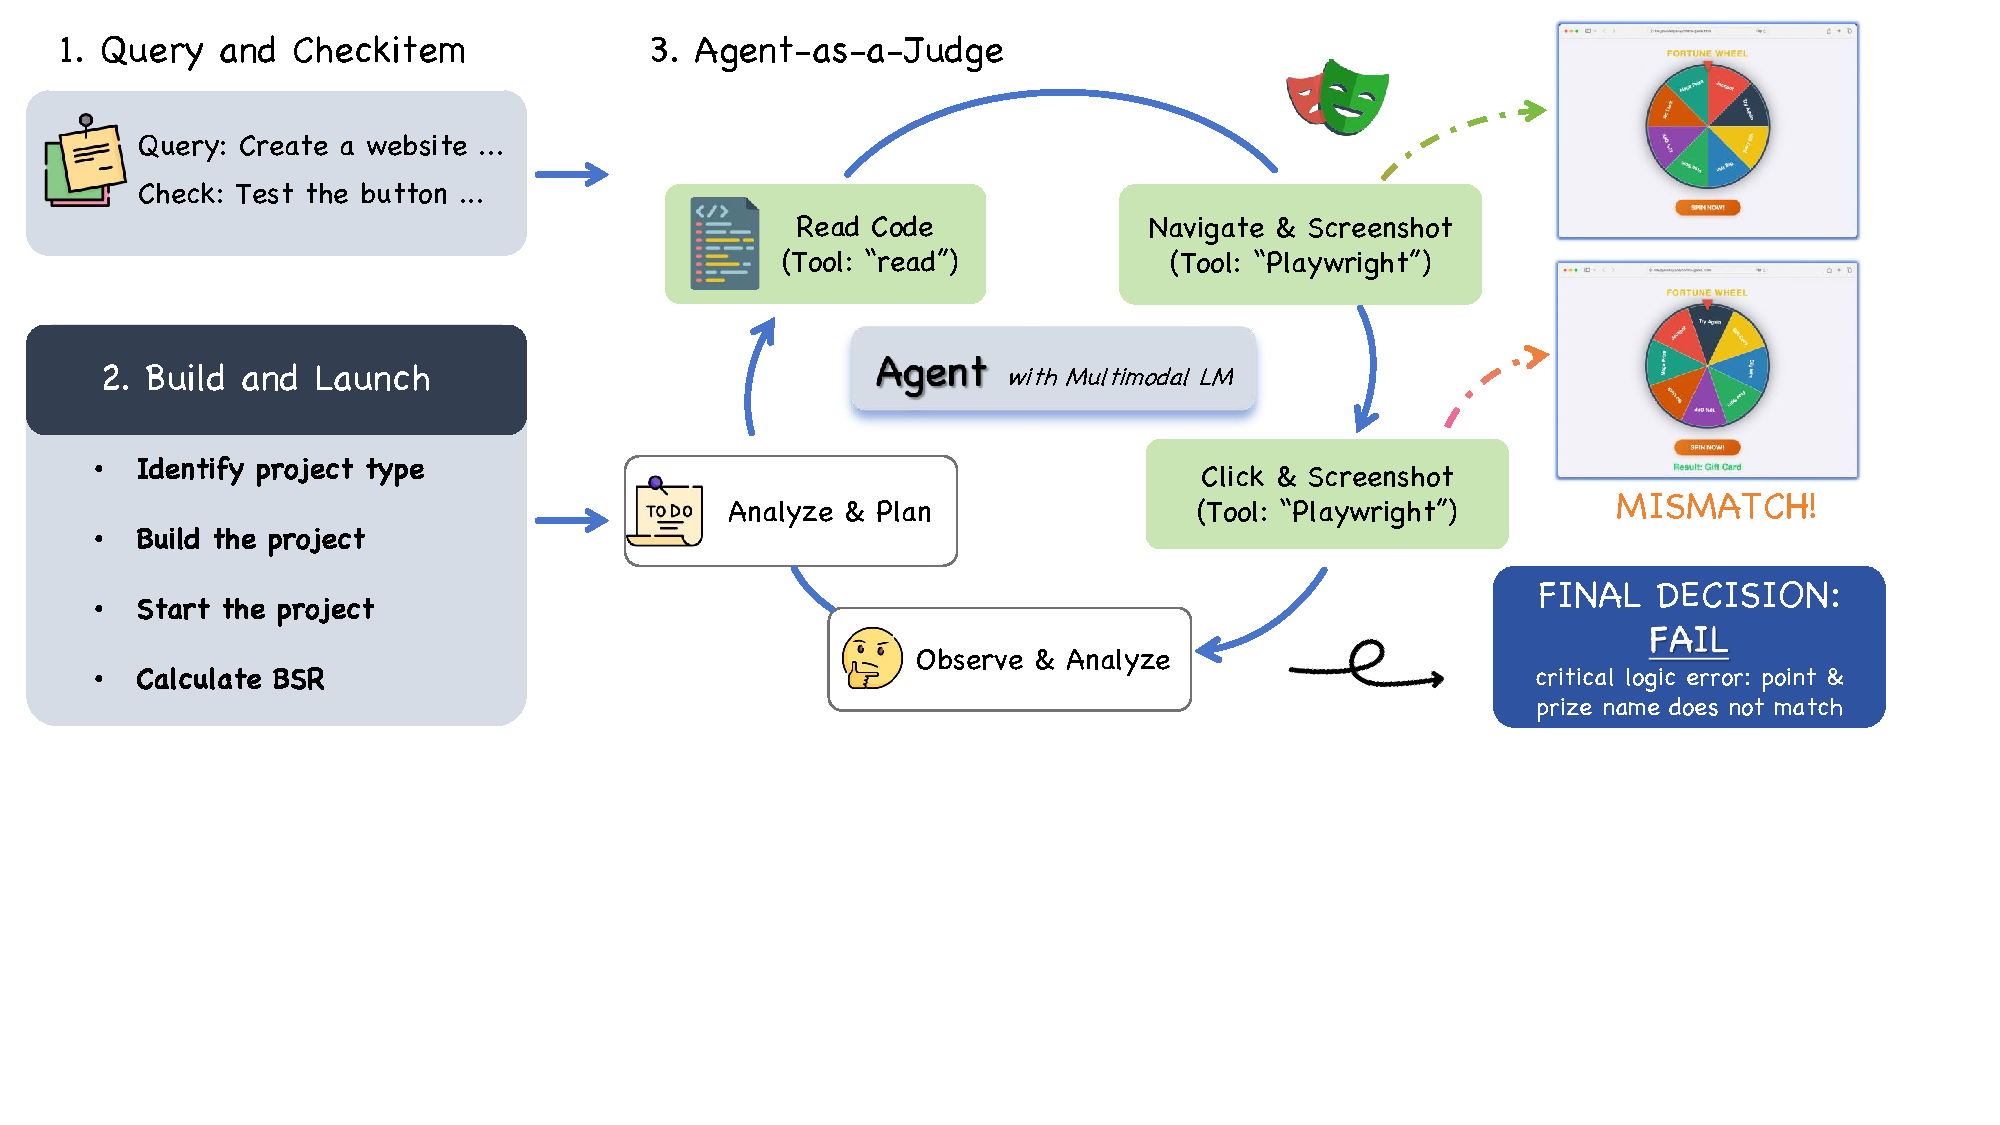
\includegraphics[width=1\linewidth]{figures/agent-as-judge.pdf}
    \vspace{-25mm}
    \caption{Agent-as-a-Judge evaluation pipeline. Each generated frontend project is first built to verify static correctness. Successfully built instances are then interactively tested by an autonomous Judge Agent, which determines the functional correctness of each check item.}
    \label{fig:agent-as-judge}
\end{figure}

\paragraph{Agent-as-a-Judge.}
Frontend correctness is inherently visual and interactive, i.e., bugs often surface only when a user clicks a button or resizes a window, making static analysis and fixed test suites insufficient. We therefore introduce Agent-as-a-Judge (Figure~\ref{fig:agent-as-judge}): each generated project is deployed in a Docker container and built to verify static correctness. Successfully built instances are then handed to an autonomous Judge Agent (Claude Code with Claude Sonnet 4.5, equipped with Playwright MCP tool) that operates in closed-loop cycles: for each check-item, the agent reads source code, interacts with the live UI (clicks, keystrokes, screenshots), inspects terminal output, and renders a pass/fail verdict.

To validate reliability, we compare Agent-as-a-Judge verdicts against independent human expert judgments along two dimensions. For \emph{point-wise consistency}, we sampled 130 check-items, had human experts score each independently, and compared against the agent's verdicts: the two agree on 94\% of items, with disagreements concentrated on subjective visual-quality criteria rather than functional specifications. For \emph{ranking consistency}, we evaluated 8 frontier models (Claude Sonnet 4.5, Claude Opus 4.5, Gemini 3 Pro, GLM-4.7, DeepSeek-V3.2, etc.) using both the automated framework and human experts. The resulting model rankings achieve a Spearman correlation of 85.7\%, indicating a strong positive correlation.

As shown in Table~\ref{tab:cc-bench-v2}, GLM-5 achieves 98.0\% BSR and is competitive with Claude Opus 4.5 in CSR, yet a notable ISR gap persists in all three stacks, indicating that GLM-5 meets most individual requirements but still falls short of Claude Opus 4.5 in completing an entire task end-to-end.

\subsubsection{Backend Evaluation}

Backend evaluation measures whether a coding agent can make correct, test-passing modifications to real-world server-side codebases under realistic engineering constraints. We curate 85 tasks spanning six languages (Python, Go, C++, Rust, Java, and TypeScript) covering domains such as search engines, database engines, web frameworks, AI inference services, knowledge management systems, and standalone algorithmic and systems-programming challenges. Task types include feature implementation, bug fixing, regression repair, and performance optimization, reflecting the diversity of day-to-day backend development.

To enable fully automated evaluation, each task is equipped with human-crafted unit tests (5--10 per task) that verify both functional correctness and edge-case handling. Tasks are packaged in a terminal-bench style: each runs inside a Docker container initialized from the project's actual build environment, and the agent receives a natural-language problem statement describing the required change. We report Pass@1, where a task is considered solved only if all its associated unit tests pass. The strict all-or-nothing criterion makes this benchmark particularly challenging: GLM-5 and Claude Opus 4.5 perform comparably (Table~\ref{tab:cc-bench-v2}), both significantly ahead of GLM-4.7.

\subsubsection{Long-horizon Evaluation}

Long-horizon evaluation targets the capabilities that distinguish production-grade agentic engineering from single-turn vibe coding: navigating massive codebases and executing multi-step development where each action reshapes the context for subsequent ones. We decompose this into two complementary tasks.

\textbf{Large Repo Exploration.} A prerequisite for any non-trivial coding task is the ability to locate the right source files in a large, unfamiliar repository. We construct an automated benchmark over real high-star GitHub repositories containing tens of thousands of files. Each question is phrased in natural, user-facing language at the level of business semantics, strictly avoiding any mention of filenames, class names, or function names. Moreover, questions require one or two hops of logical reasoning from the user-facing description to the actual implementation---for instance, a question about misaligned lip-sync in a generated video maps to a parameter-tuning block inside a video generation backend. Target files are selected to maximize navigation difficulty: they reside at least three directory levels deep, carry opaque names that resist keyword-based search, implement unique functionality not duplicated elsewhere in the repository, and lie outside its main feature surface. We report Pass@1 averaged over three runs, where a question is considered solved if the agent successfully reads the target file during exploration. In this task, GLM-5 outperforms Claude Opus 4.5 (Table~\ref{tab:cc-bench-v2}), both far ahead of GLM-4.7. The result suggests that effective repo exploration depends less on raw code generation ability and more on strategic search, i.e., iteratively narrowing the file space via directory-level reasoning and semantic association, where GLM-5's training on agentic tool-use trajectories provides a clear advantage.

\textbf{Multi-step Chained Tasks.} Mainstream coding benchmarks such as SWE-bench reduce evaluation to single-commit, isolated edits, and therefore cannot assess an agent's ability to perform incremental development where each step alters the codebase state for subsequent steps. To address this, we construct a long-horizon benchmark by mining merged Pull Requests from high-quality repositories and assembling task chains via the following pipeline:

\begin{enumerate}[leftmargin=1.5em,itemsep=2pt]
    \item \textbf{PR Filtering.} Retain only merged PRs that include tests, contain 3--15 commits, and follow a linear (non-merge) history.
    \item \textbf{Semantic Grouping.} An LLM scores pairwise semantic relatedness between adjacent commits; dynamic programming finds the optimal partition into coherent task groups that maximize intra-group coherence while preserving commit order.
    \item \textbf{Patch Triage.} Each task's cumulative diff is split into three categories: \emph{golden patch} (core code the agent must produce), \emph{test patch} (verification tests), and \emph{auto-apply patch} (configuration and fixtures applied automatically).
    \item \textbf{Problem Statement Generation.} An LLM generates a natural-language problem statement for each task from its patch and commit messages.
    \item \textbf{Task Classification.} Tasks are automatically classified (feature / bug-fix / refactor / test / config) and evaluated along three axes: error elimination, critical-path accuracy, and test passage.
    \item \textbf{Environment Validation.} Docker environments are constructed, and golden patches are applied to verify zero regression across the entire chain.
\end{enumerate}

Given a chain of $K$ tasks, the agent starts from the base commit and works sequentially: after completing task $k$, its changes are committed, and the auto-apply patch for task $k{+}1$ is applied, so the codebase state evolves cumulatively. Evaluation checks each commit in turn and cumulatively applies test patches from tasks $1$ through $k$ before running the full test suite, catching both failures on the current task and regressions on earlier ones. We report Pass@1 on individual tasks. This chained and state-recursive design directly evaluates the long-range context tracking, planning, and incremental development abilities that single-commit benchmarks leave untested. As Table~\ref{tab:cc-bench-v2} shows, GLM-5 improves substantially over GLM-4.7, but a significant gap to Claude Opus 4.5 remains. This is because errors are compounded across the chain: a suboptimal edit in one task can silently break tests in subsequent tasks. Narrowing this gap will require advances in long-context consistency and long-horizon self-correction, both active areas of our ongoing research.


\subsubsection{Evaluation on evolving SWE tasks}
We evaluate on SWE-rebench~\cite{badertdinov2025swe} because SWE-bench Verified is a static, public, human-validated test set and released for more than 2 years. In contrast, SWE-rebench is built on an automated pipeline that continuously mines fresh, real GitHub issue-fixing tasks, enabling decontaminated, time-robust evaluation that better measures generalization to new software engineering problems rather than performance on a static benchmark. Table~\ref{table:swe_rebench} shows the official performance of GLM-5 on SWE-rebench and we observe that GLM-5 can effectively generalize to new SWE problems.


\begin{table}[t]
\centering
\caption{Performance on SWE-rebench, January 2026.}
\begin{tabular}{lccc}
\toprule
Model & Resolved Rate (\%) & Resolved Rate SEM ($\pm$, \%) & Pass@5 (\%) \\
\midrule
Claude Opus 4.6 & 52.9\% & 1.06\% & 70.8\% \\
GPT-5.2 (xhigh) & 51.7\% & 1.21\% & 58.3\% \\
Claude Sonnet 4.5 & 47.1\% & 1.69\% & 60.4\% \\
Gemini 3 Pro & 46.7\% & 2.04\% & 58.3\% \\
Claude Opus 4.5 & 43.8\% & 0.93\% & 58.3\% \\
GLM-5 & 42.1\% & 1.21\% & 50.0\% \\
GLM-4.7 & 41.3\% & 2.12\% & 56.3\% \\
% MiniMax M2.5 & 39.6\% & 0.66\% & 56.3\% \\
Kimi K2.5 & 37.9\% & 1.21\% & 50.0\% \\
\bottomrule
\end{tabular}
\label{table:swe_rebench}
\end{table}


\subsection{Evaluation of Real-world General Abilities}

\begin{figure}
    \centering
    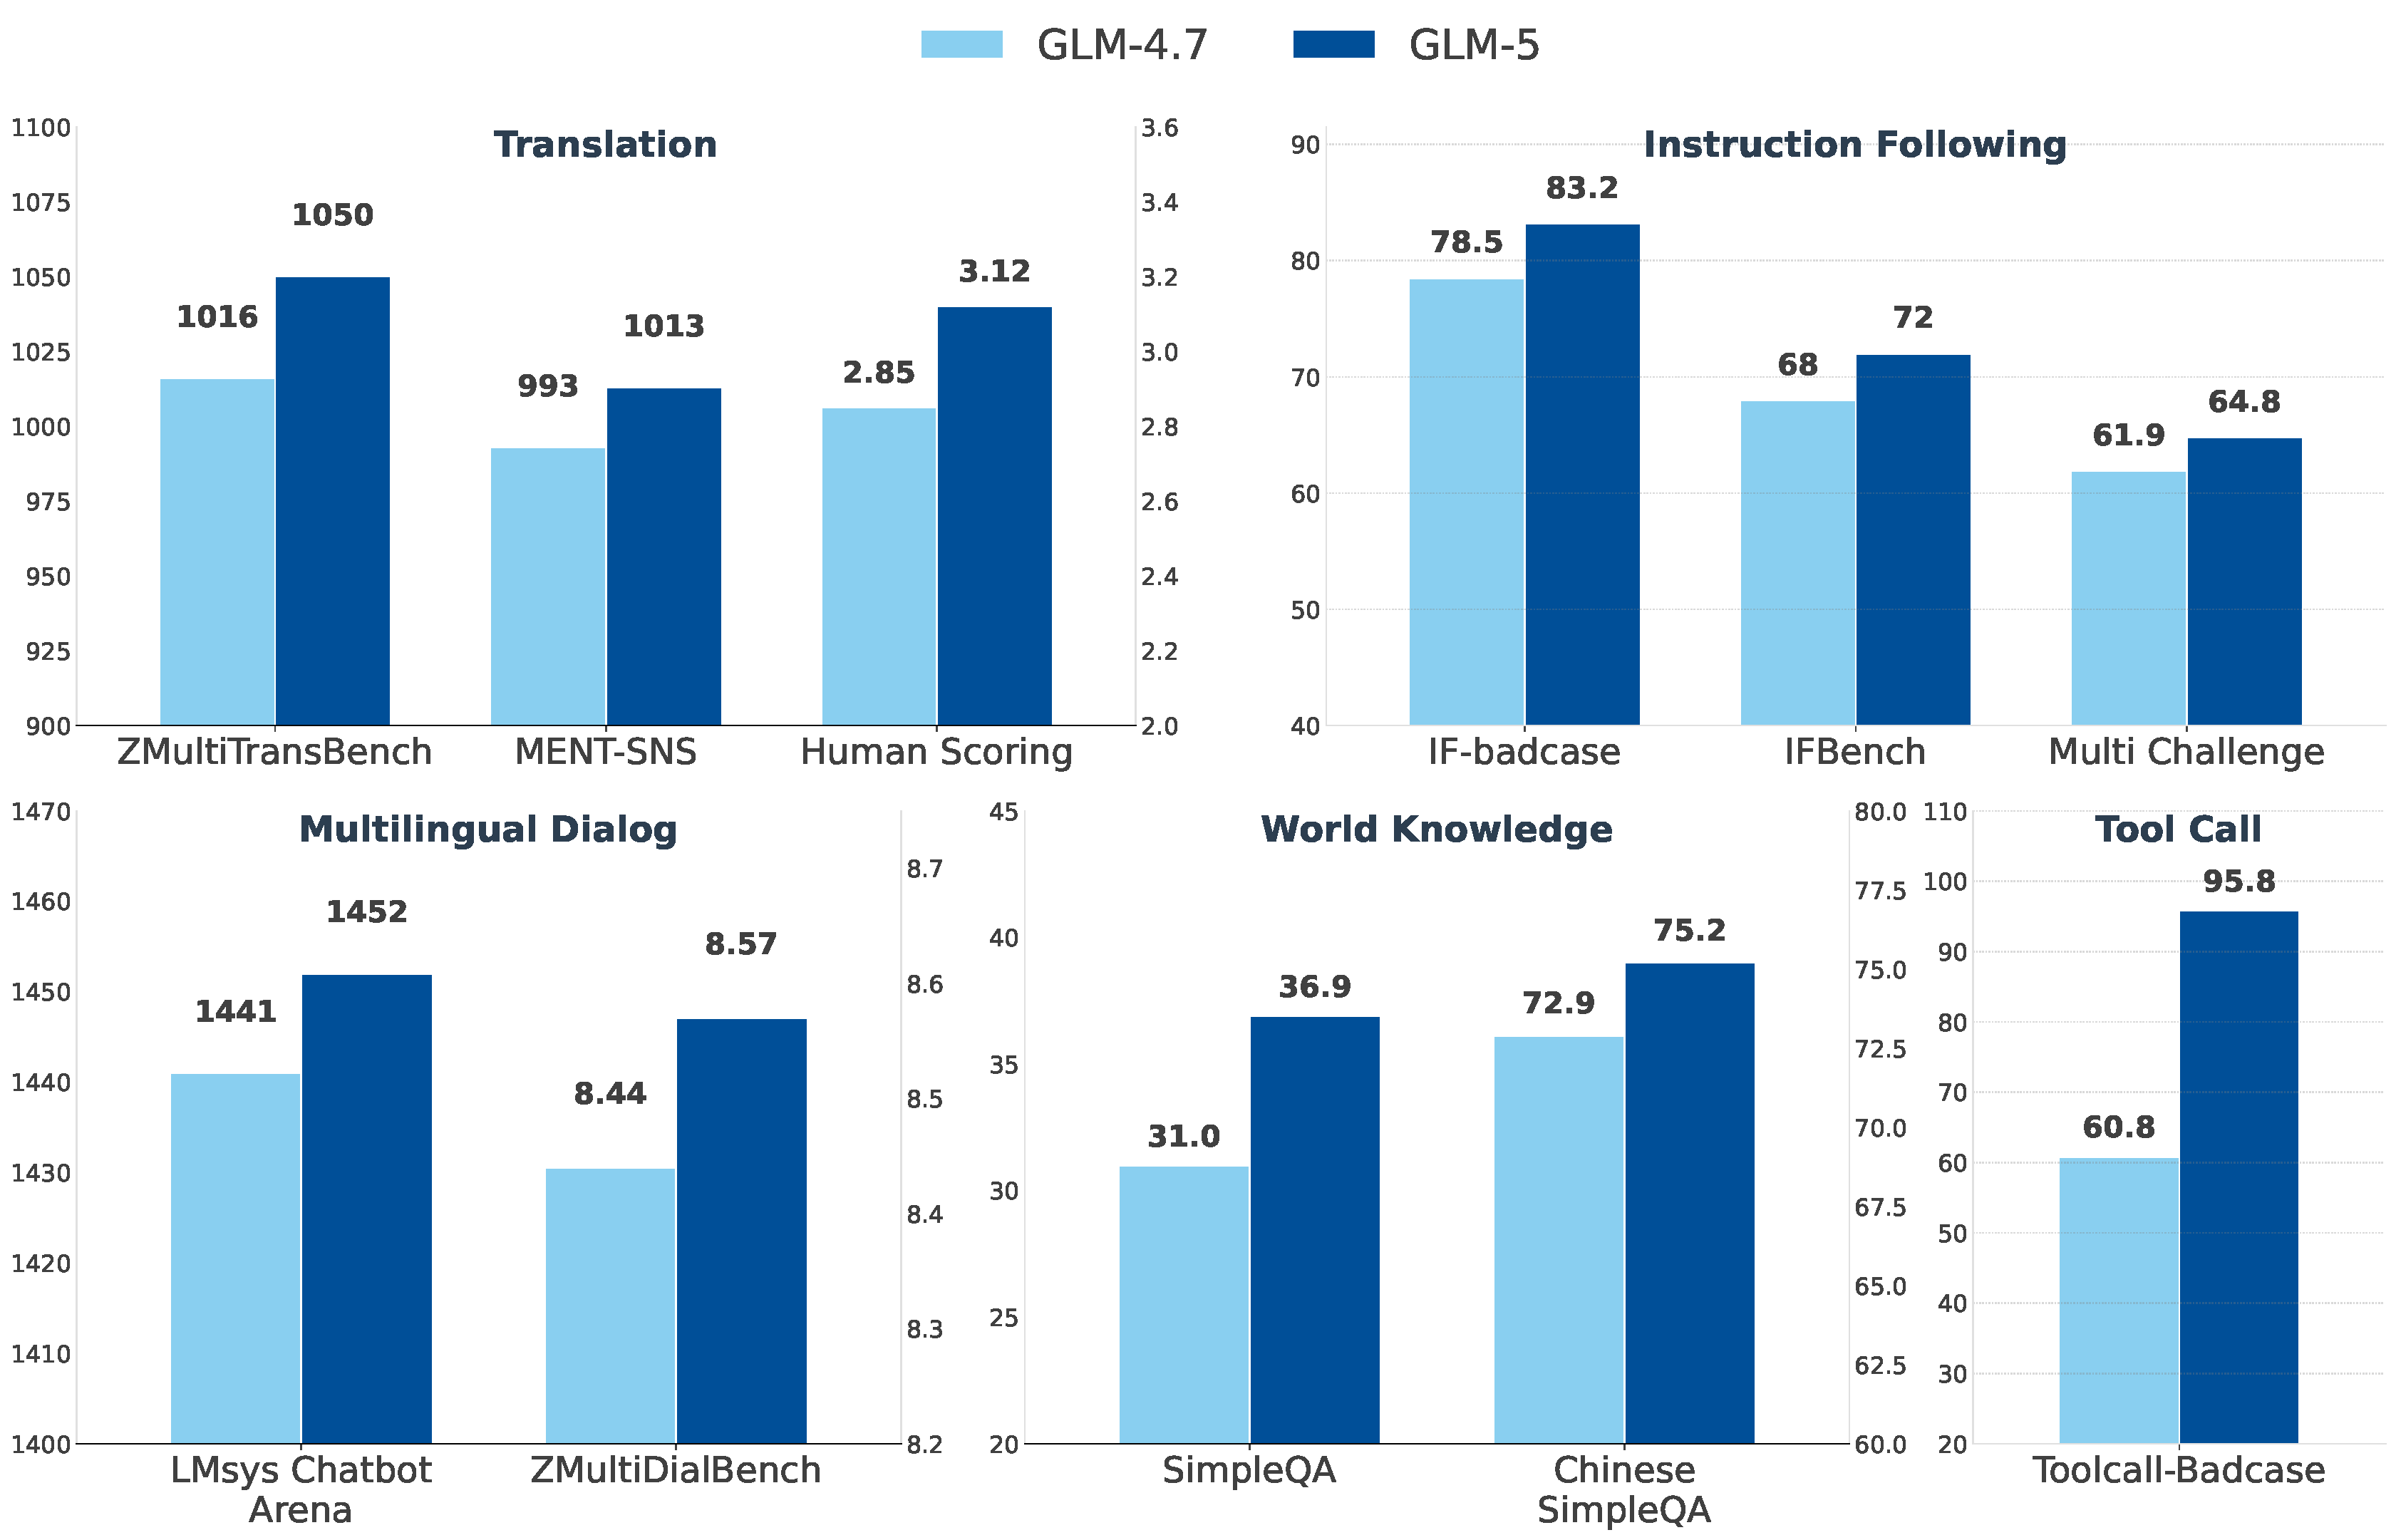
\includegraphics[width=1\linewidth]{figures/glm5_realscene_comparison.pdf}
    \caption{Performance comparison between GLM-4.7 and GLM-5 across five real-world general ability domains.}
    \label{fig:glm5_realscene}
\end{figure}

While standardized academic benchmarks provide useful signals, they do not fully capture how models are used in practice. To recognize this gap, we evaluate GLM-5 on a set of real-world general abilities derived from high-frequency user interaction patterns observed in deployment settings. These abilities include {machine translation, multilingual dialogue, instruction following, world knowledge, and tool-calling}.

Unlike traditional benchmark-centric evaluation, our goal is to measure improvements that directly translate into user-perceived quality gains. For each capability, we adopt a combination of internal human evaluation, internal automated evaluation, external human assessment, and external automated benchmarks, ensuring both diagnostic granularity and cross-model comparability. When using external benchmarks, we prioritize datasets that reflect realistic interaction patterns rather than narrowly constructed test distributions.

Figure~\ref{fig:glm5_realscene} presents the comparative results between GLM-5 and GLM-4.7 across five real-world capability domains. Across all evaluated dimensions, GLM-5 shows consistent improvements in machine translation, multilingual dialogue, instruction following, world knowledge, and tool-calling.


Detailed evaluation protocols and dataset descriptions for each ability are provided as follows. % in the following subsections.

\subsubsection{Machine Translation}

\paragraph{ZMultiTransBench.} 
This internal dataset comprises 1,220 samples sourced from self-collected high-frequency translation scenarios, covering seven language pairs: Zh to Es (\(300\)), Ru (\(250\)), Fr (\(220\)), Ko (\(200\)), Ja (\(150\)), Ar (\(50\)), and De (\(50\)). All samples were curated, translated, and independently verified by graduate students with formal training in translation studies. The dataset emphasizes naturally occurring usage contexts rather than artificially constructed test cases. Evaluation is conducted using pairwise comparison against a fixed baseline response. Judgments are provided by an automated evaluator based on GPT-4.1, which assesses semantic fidelity, fluency, and overall translation quality.


\paragraph{MENT-SNS.}
To further evaluate robustness in linguistically challenging contexts, we adopt source sentences from MENT \citep{tian2026ment}, comprising \(753\) English–Chinese sentence pairs across four domains: Social Network Services (SNS), Cross-Culture, Poetry, and Literature.
These domains are selected to stress-test translation under complex linguistic phenomena, including slang, homophonic wordplay, idiomatic expressions, historical references, and metaphorical language. Similar to ZMultiTransBench, all samples were curated and verified by professionally trained graduate students.
Evaluation follows the same pairwise comparison protocol against a baseline response, with GPT-4.1 serving as the automated judge model.

\subsubsection{Multi-lingual Dialogue}
\paragraph{LMArena.}
We report Elo ratings from the LMArena\footnote{https://arena.ai/leaderboard/text}
, which are derived from large-scale, community-submitted pairwise comparisons. These ratings reflect relative model preference in open-ended dialogue settings and provide an external signal of conversational performance. %, deployment-proximal 

\paragraph{ZMultiDialBench.}
In addition to the public leaderboard, we also conduct human evaluation on ZMultiDialBench, an internal multilingual dialogue benchmark. The dataset consists of 141 curated instances spanning diverse dialogue categories. Samples were collected from high-quality conversational data contributed by native-speaking annotators across multiple countries, as well as from challenging failure cases reported by online users. 
Human annotators assigned pointwise scores on a 1–10 scale to anonymized model responses according to category-specific, standardized evaluation criteria. 

\subsubsection{Instruction Following}
\paragraph{IF-Badcase.} IF-Badcase is an internal benchmark constructed from instruction-following \textbf{failure cases} reported by real users in production settings. The dataset is designed to evaluate strict adherence to realistic, multi-constraint instructions, emphasizing procedural accuracy, logical consistency, and rigid formatting requirements.
Evaluation is conducted using a detailed checklist-based protocol that verifies compliance with explicit constraints, including ordered steps, rule-based conditions, and structural specifications. All samples were annotated, reviewed, and iteratively filtered by human experts, resulting in a curated set of 450 test instances.

\paragraph{IF-Bench~\citep{ifbench}.} IF-Bench evaluates LLMs on their ability to adhere to complex, objective constraints, such as specific formatting rules, length limits, and content restrictions. It provides a quantitative measure of precise instruction-following capabilities, focusing on verifiable compliance rather than open-ended generation quality.

\paragraph{MultiChallenge~\citep{multichallenge}.} MultiChallenge examines LLMs via realistic, multi-turn conversational scenarios. It targets complex interactions requiring accurate instruction-following, context allocation, and in-context reasoning.


\subsubsection{World Knowledge}

\paragraph{SimpleQA~\citep{simpleQA}.} SimpleQA measures short-form factuality using challenging questions with single, indisputable answers. It evaluates a model's calibration by classifying responses as correct, incorrect, or not attempted, prioritizing accuracy over generation length.

\paragraph{Chinese SimpleQA~\citep{chinesesimpleQA}.} Adapting the SimpleQA methodology to the Chinese context, this benchmark evaluates factuality across six major domains and 99 subtopics. It utilizes high-quality, static, short-answer questions designed for reliable, automated grading to assess the knowledge accuracy of LLMs.

\subsubsection{Tool Calling}
\paragraph{ToolCall-Badcase.} ToolCall-Badcase is an internal benchmark derived from \textbf{failure cases} in tool invocation scenarios reported by users in production environments. Each instance is associated with a verifiable ground-truth tool call, enabling objective evaluation of both tool selection and argument correctness.
Evaluation assesses whether the model (1) invokes the correct tool and (2) provides correctly structured and semantically accurate arguments. 
All samples underwent multiple rounds of review, rewriting, and validation to remove ambiguity and ensure evaluability. The resulting dataset consists of 200 curated test cases that reflect realistic tool-calling abilities.